% !TEX TS-program = pdflatex
% !TEX encoding = UTF-8 Unicode

\documentclass[portuges]{beamer}

\definecolor{darkred}{rgb}{0.5,0,0}

\mode<presentation>
{
  \usetheme{Warsaw}
  %\usecolortheme{seahorse}
  \setbeamercolor*{palette primary}{use=structure,fg=white,bg=darkred}
  \setbeamercolor*{section in toc}{fg=darkred}
  \setbeamercolor*{palette quaternary}{fg=white,bg=gray!30!black}
  \setbeamercolor*{item}{fg=red}
%  \setbeamercovered{transparent}
}

\usepackage[portuges]{babel}

\usepackage[utf8]{inputenc}

\usepackage{times}
\usepackage[T1]{fontenc}

\title
{MyStreet}

\subtitle
{Rede social para parttilha de informação sobre infraestruturas}

\author[Li4]
{
Bruno Matos nº 33147\\ 
Carlos Cosio nº 5177\\
Jorge Rodrigues nº 51751\\
Miguel Fernandes nº 44024\\ 
Rui Silva nº 47082\\
}

\date % [Short Occasion] % (optional)
{
LEI-LI4       \\
2012-2013
}

\subject{MyStreet Apresentação}
% This is only inserted into the PDF information catalog. Can be left
% out. 

% Logo
%\pgfdeclareimage[height=0.5cm]{university-logo}{LogoUM.jpg}
%{\pgfuseimage{university-logo}}
\logo{
   
\includegraphics[height=0.5cm]{LogoUM.jpg}
   }

% Delete this, if you do not want the table of contents to pop up at
% the beginning of each subsection:
\AtBeginSubsection[]
{
  \begin{frame}<beamer>{}
    \tableofcontents[currentsection,currentsubsection]
  \end{frame}
}


% If you wish to uncover everything in a step-wise fashion, uncomment
% the following command: 

\beamerdefaultoverlayspecification{<+->}

\begin{document}

\begin{frame}
  \titlepage
\end{frame}

\begin{frame}{Visão Geral}
  \tableofcontents
  % You might wish to add the option [pausesections]
\end{frame}


% Since this a solution template for a generic talk, very little can
% be said about how it should be structured. However, the talk length
% of between 15min and 45min and the theme suggest that you stick to
% the following rules:  

% - Exactly two or three sections (other than the summary).
% - At *most* three subsections per section.
% - Talk about 30s to 2min per frame. So there should be between about
%   15 and 30 frames, all told.

\section{Introdução}

\subsection{Problema}

\begin{frame}{Descrição}
  \begin{itemize}
  \item Monitorização de infraestruturas numa determinada zona
  \item Tempo longo na deteção de problemas
  \item Falta de comunicação com os moradores
  \item Necessidade de deslocação ao local
  \end{itemize}
\end{frame}

\subsection{Soluções}

\begin{frame}{Soluções Possíveis}
  \begin{itemize}
  \item Nomeação de um representante local
  \item Atribuição de zonas a equipas de manutenção
    \begin{itemize}
    \item Circuitos diários
    \item Recolha de informação junto dos moradores
    \end{itemize}
  \item \textbf{Criação de uma rede social}
  \end{itemize}
\end{frame}

\begin{frame}{Solução Escolhida}{Criação de uma rede social}
  \begin{itemize}
  \item Comunicação feita através da internet
  \item Baseada no modelo de redes sociais conhecidas
  \item Possibilita o contacto direto entre moradores e funcionários
  \item Possibilidade de utilização de dispositivos móveis
  \end{itemize}
\end{frame}

\subsection{Objetivos}

\begin{frame}{Gerais}
 \begin{itemize}
 \item Facilitar a comunicação entre comunidades locais e responsáveis técnicos
 \item Fomentar a troca de ideias entre moradores
 \item Simplificar a monitorização de infraestrtuturas
 \end{itemize}
\end{frame}

\begin{frame}{Aplicação}
 \begin{itemize}
 \item Simples e fácil de usar
 \item Estar disponível 24h/dia
 \item Utilizar tecnologia de ponta
 \item Suporte para várias plataformas
 \item Fácil integração com outros serviços 
 \end{itemize}
\end{frame}

\section{Requisitos}

\subsection{Atores}

\begin{frame}{Atores}
 \begin{itemize}
 \item Moradores
 \item Funcionários
 \item Administradores
 \end{itemize}
\end{frame}

\subsection{Funcionalidades}

\begin{frame}{Moradores}
 \begin{itemize}
 \item Reportar ocorrência
 \item Classificar intervenção
 \end{itemize}
\end{frame}

\begin{frame}{Funcionários}
 \begin{itemize}
 \item Atualizar ocorrência
 \item Fechar ocorrência
 \end{itemize}
\end{frame}

\begin{frame}{Moradores e Funcionários}
 \begin{itemize}
 \item Adicionar comentários	
 \item Criar e editar perfil
 \item Autenticar-se
 \item Consultar ocorrências
 \item Consultar estatísticas
 \end{itemize}
\end{frame}

\begin{frame}{Administradores}
 \begin{itemize}
 \item Definir funcionários
 \item Eliminar ou bloquear utilizadores
 \end{itemize}
\end{frame}

\section{Desenvolvimento}

\subsection{Arquitetura}

\begin{frame}{Componentes}
 \begin{itemize}
 \item Base de dados
 \item Web service
 \item Aplicação Web
 \item Aplicação Mobile 
 \end{itemize}
\end{frame}

\subsection{Componentes}

\begin{frame}{Base de dados}
 \begin{itemize}
 \item Persistência de toda a informação do sistema
 \item MS SQL Server 2012
 \begin{itemize}
  \item Fiabilidade
  \item Rapidez
  \item Funcionalidades
 \end{itemize}
 \item Gerada pela Entity Framework
 \end{itemize}
\end{frame}

\begin{frame}{Web service}
 \begin{itemize}
 \item Interface com a base de dados utilizando a Entity Framework
 \item Lógica de negócio
 \item REST (Representational State Transfer)
 \item .NET Framework - Web Api 
 \end{itemize}
\end{frame}

\begin{frame}{Lista de Ocorrências}
 \begin{center}
  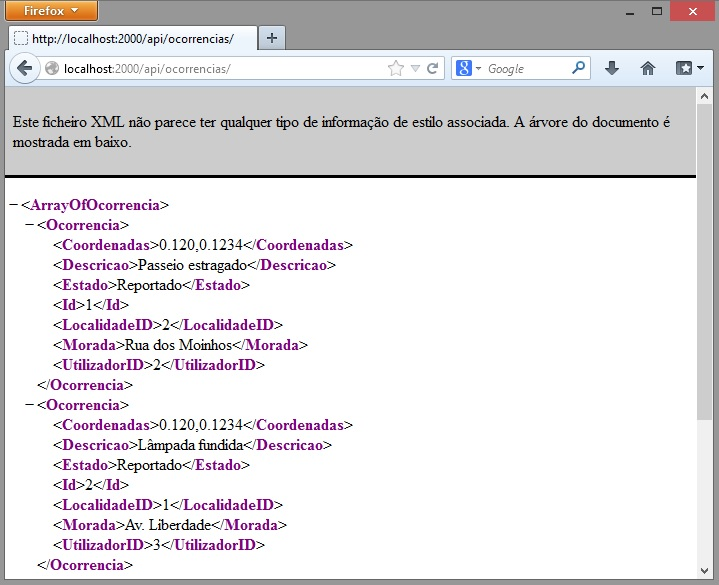
\includegraphics[height=5cm]{ocorrencias.jpg}
 \end{center}
\end{frame}

\begin{frame}{Detalhes de uma Ocorrência}
 \begin{center}
  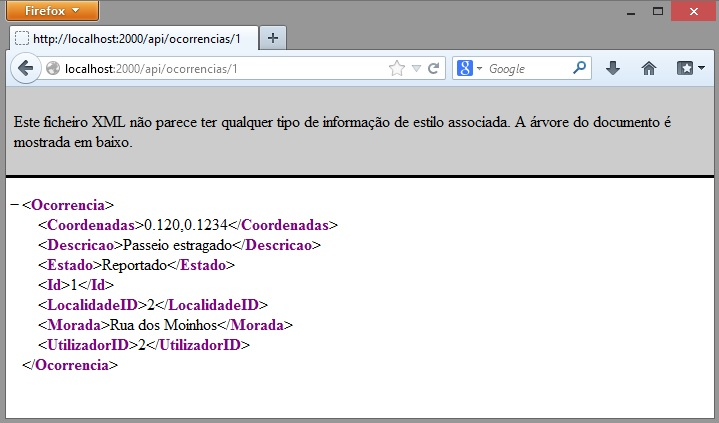
\includegraphics[height=5cm]{ocorrencia.jpg}
 \end{center}
\end{frame}

\begin{frame}{Aplicação Web}
 \begin{itemize}
 \item Principal interface com o utilizador
 \item Implementação de todas as funcionalidades do sistema
 \item Utilização de AJAX
 \item ASP.NET 
 \item Mapas: OpenLayers
 \end{itemize}
\end{frame}

\begin{frame}{Aplicação Mobile}
 \begin{itemize}
 \item Android
 \item Implementação de um subconjunto alargado das funcionalidades do sistema
 \item Utilização de JSON
 \item Android
 \item Aplicação nativa
 \begin{itemize}
  \item Interação com GPS
  \item Interação com o dispositivo de captura de imagem
  \item Framework madura e bastante completa
 \end{itemize}
 \end{itemize}
\end{frame}

\section*{Conclusões}

\begin{frame}{Conclusões}

  \begin{itemize}
  \item Metodologias de trabalho são fundamentais
  %\item A organização do grupo de trabalho é uma peça central no sucesso do mesmo
  \item As tecnologias emergentes podem ter um papel fundamental na velociade e facilidade do desenvolvimento
  \item Um bom processo de desenvolvimento pode ter resultados interessantes até num curto espaço de tempo 
  \end{itemize}
  
  % The following outlook is optional.
  \vskip0pt plus.5fill
  \begin{itemize}
  \item
    Passos seguintes
    \begin{itemize}
    \item Possível interação com \emph{software} existente 
    \item Internacionalização
    \end{itemize}
  \end{itemize}
\end{frame}


\end{document}


